% Name: GRU cell
% Description: A gated recurrent unit: the reset gate r scales the old state before the candidate, and the update gate z blends the old state with the candidate.
% Tags: GRU, recurrent network, gates, sequence model

\usetikzlibrary{arrows.meta}

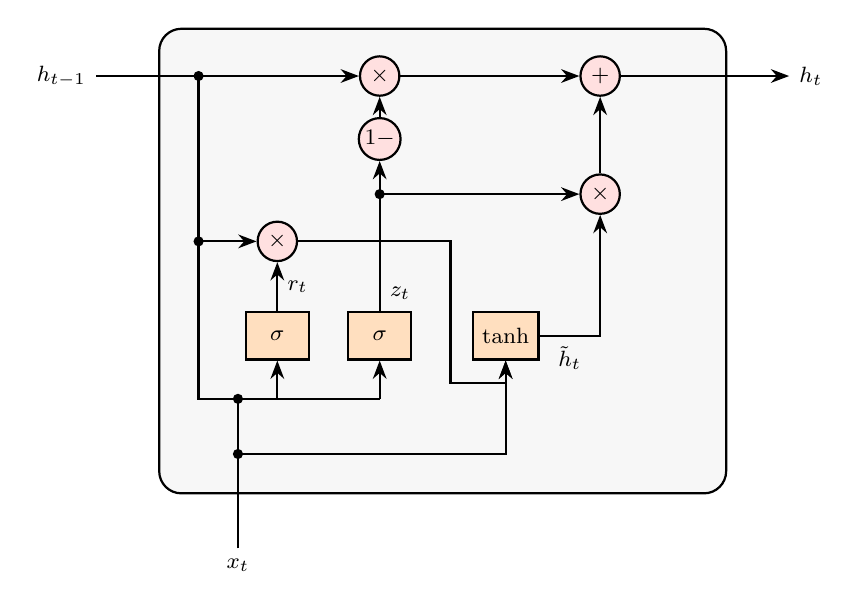
\begin{tikzpicture}[>={Stealth}, thick, every node/.style={font=\footnotesize},
    gate/.style={draw, fill=orange!25, minimum width=8mm, minimum height=6mm},
    op/.style={circle, draw, fill=red!12, inner sep=0pt, minimum size=5mm},
    dot/.style={circle, fill, inner sep=1.3pt}]
  \draw[rounded corners=8pt, fill=gray!6] (0,-0.9) rectangle (7.2,5);
  \node[gate] (r) at (1.5,1.1) {$\sigma$};
  \node[gate] (z) at (2.8,1.1) {$\sigma$};
  \node[gate] (g) at (4.4,1.1) {$\tanh$};
  \node[op] (mr) at (1.5,2.3) {$\times$};
  \node[op, inner sep=1pt] (one) at (2.8,3.6) {$1-$};
  \node[op] (m1) at (2.8,4.4) {$\times$};
  \node[op] (mz) at (5.6,2.9) {$\times$};
  \node[op] (add) at (5.6,4.4) {$+$};
  % h_t = (1 - z) h_{t-1} + z times the candidate.
  \draw[->] (-0.8,4.4) node[left] {$h_{t-1}$} -- (m1);
  \draw[->] (m1) -- (add);
  \draw[->] (add) -- (8,4.4) node[right] {$h_t$};
  \draw (0.5,4.4) node[dot] {} -- (0.5,0.3) -- (2.8,0.3);
  \draw[->] (0.5,2.3) node[dot] {} -- (mr);
  \draw (1,-1.6) node[below] {$x_t$} -- (1,0.3) node[dot] {};
  \foreach \n in {r, z} \draw[->] (\n |- 0,0.3) -- (\n);
  \draw[->] (r) -- node[right] {$r_t$} (mr);
  \draw[->] (z) -- node[pos=0.12, right] {$z_t$} (one);
  \draw[->] (one) -- (m1);
  \draw[->] (2.8,2.9) node[dot] {} -- (mz);
  % The candidate sees the reset old state and the input.
  \draw[->] (mr) -- (3.7,2.3) |- (4.4,0.5) -- (g);
  \draw[->] (1,-0.4) node[dot] {} -| (g);
  \draw[->] (g) -| node[pos=0.25, below] {$\tilde{h}_t$} (mz);
  \draw[->] (mz) -- (add);
\end{tikzpicture}
